\documentclass[a3,convert]{standalone}
\usepackage{pgfplots}
\usepgfplotslibrary{smithchart}    
\usepgfplotslibrary{polar}   
\usepackage{siunitx} 
\usepackage{tikz}
\pgfplotsset{compat=1.18}
\usetikzlibrary{calc,intersections,through}
\usepackage{comment}

\begin{document}

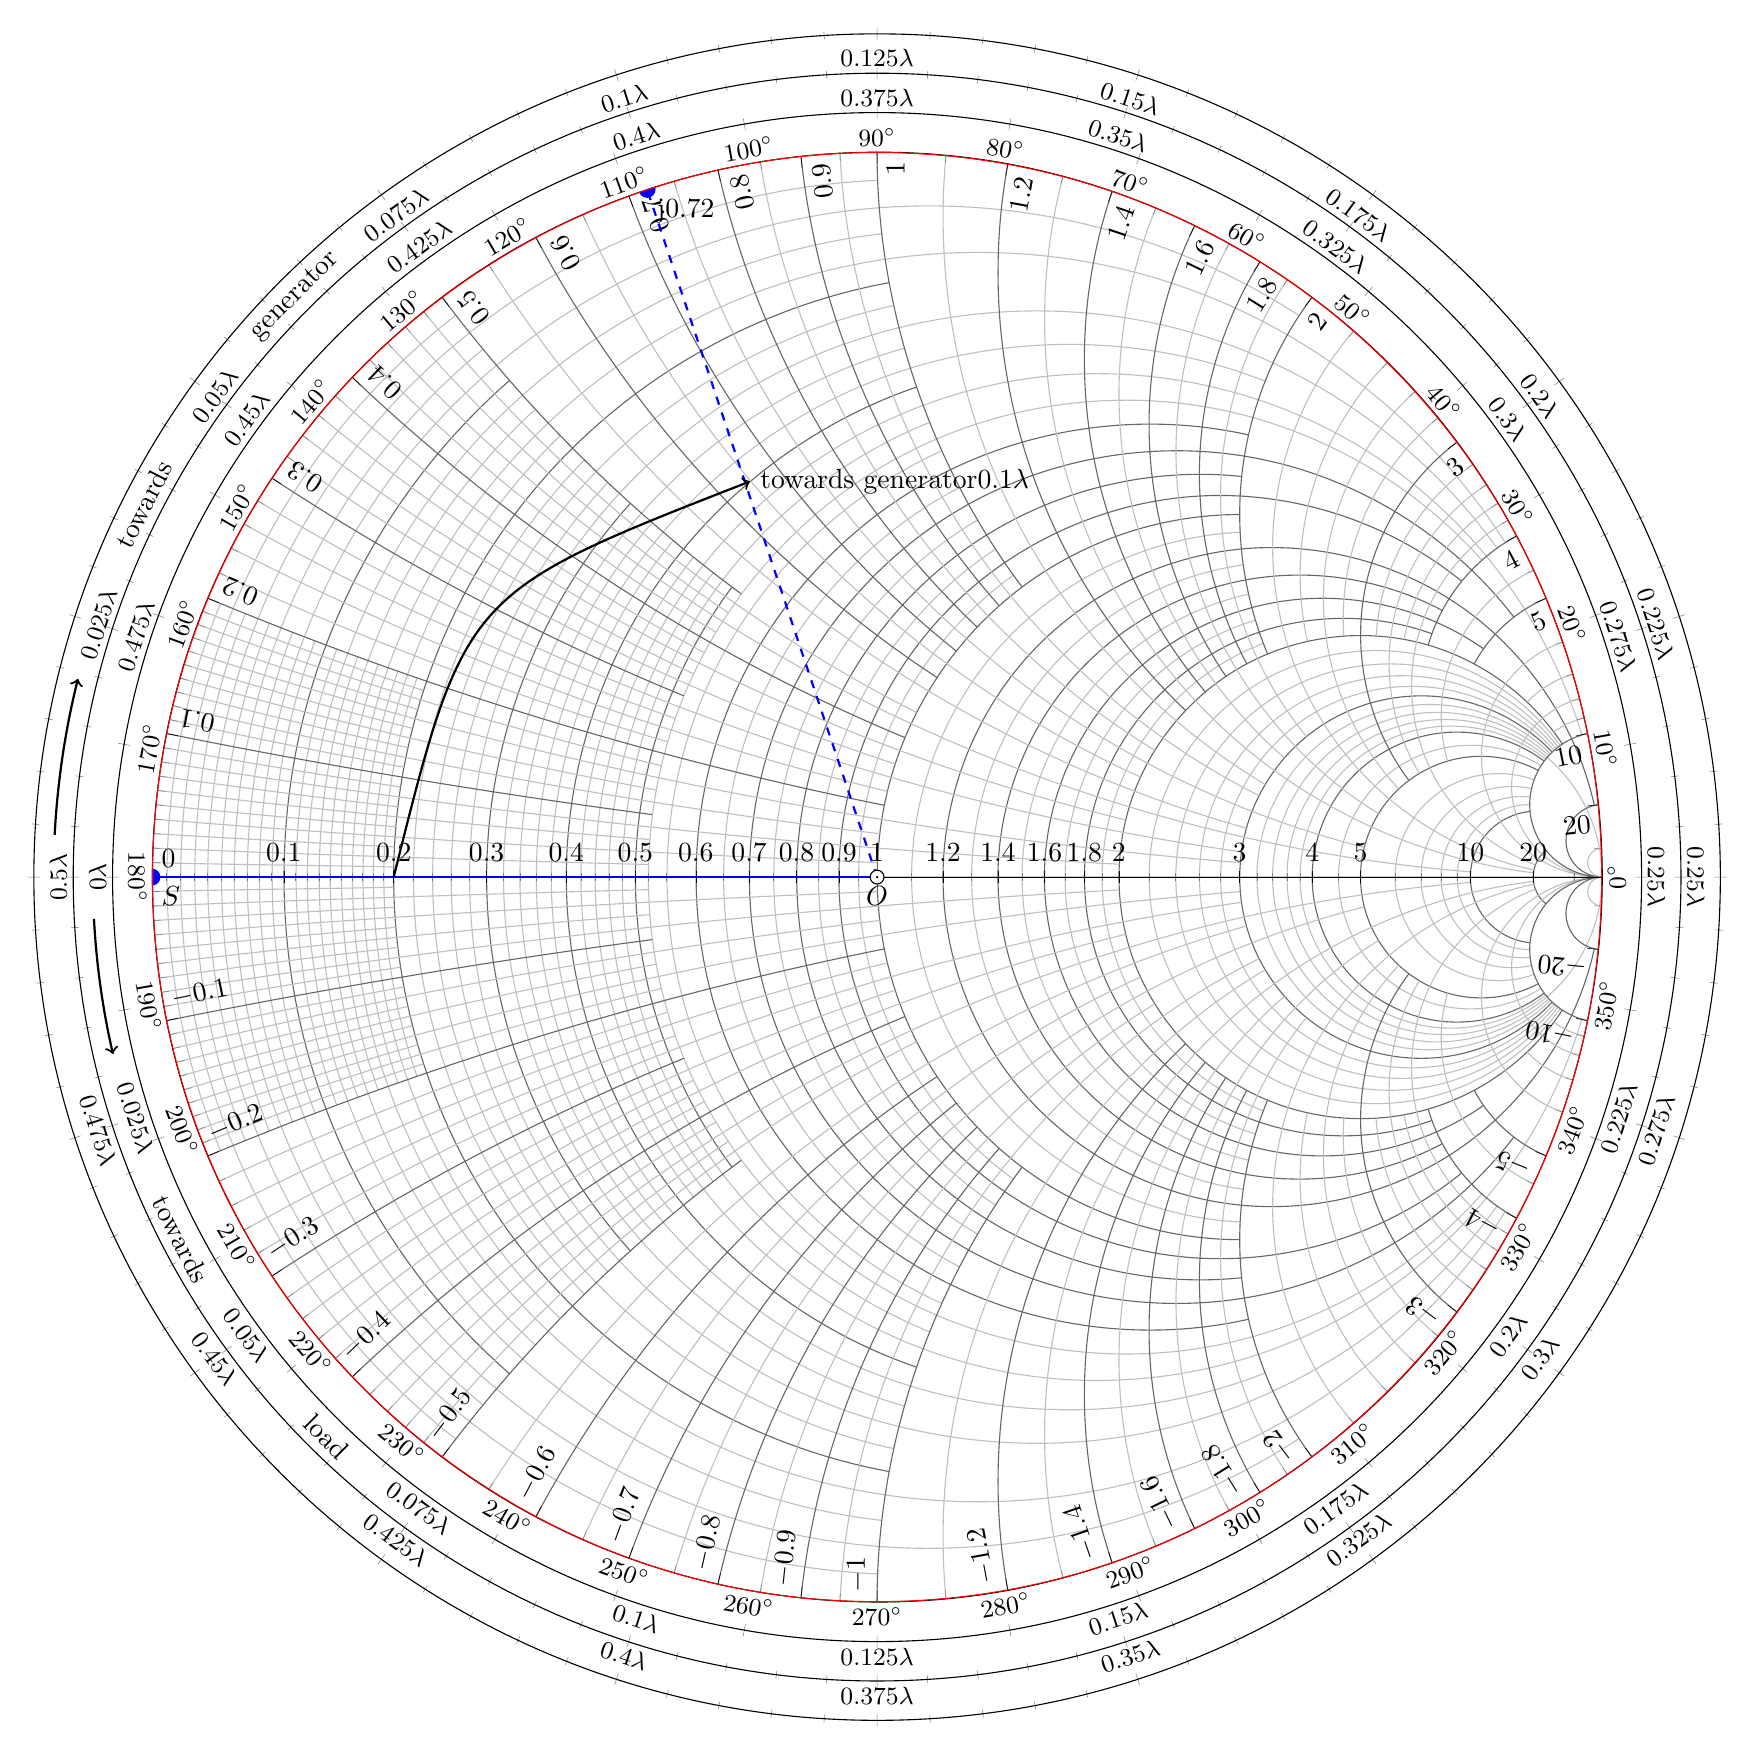
\begin{tikzpicture}
    \pgfmathsetmacro{\xoffset}{10.45*(1-cos(3))-1.25}
    \pgfmathsetmacro{\yoffset}{sin(3)*10.45+9.2}
    \draw[,thick,->] (+\xoffset,\yoffset) arc [radius=10.45cm,start angle=177,end angle=166];
    \pgfmathsetmacro{\xoffset}{10.45*(1-cos(18))-1.25}
    \pgfmathsetmacro{\yoffset}{sin(18)*10.45+9.2}
    \draw[,draw=none] (+\xoffset,\yoffset) arc [radius=10.45cm,start angle=162,end angle=144] node[midway,sloped]{towards};
    \pgfmathsetmacro{\xoffset}{10.45*(1-cos(36))-1.25}
    \pgfmathsetmacro{\yoffset}{sin(36)*10.45+9.2}
    \draw[,draw=none] (+\xoffset,\yoffset) arc [radius=10.45cm,start angle=144,end angle=126] node[midway,sloped]{generator};

    \pgfmathsetmacro{\xoffset}{9.95*(1-cos(-3))-0.75}
    \pgfmathsetmacro{\yoffset}{sin(-3)*9.95+9.2}
    \draw[,thick,->] (\xoffset,\yoffset) arc [radius=9.95cm,start angle=183,end angle=193] ;
    \pgfmathsetmacro{\xoffset}{9.95*(1-cos(-18))-0.75}
    \pgfmathsetmacro{\yoffset}{sin(-18)*9.95+9.2}
    \draw[,draw=none] (+\xoffset,\yoffset) arc [radius=10.45cm,start angle=198,end angle=216] node[midway,sloped]{towards};
    \pgfmathsetmacro{\xoffset}{9.95*(1-cos(-36))-0.75}
    \pgfmathsetmacro{\yoffset}{sin(-36)*9.95+9.2}
    \draw[,draw=none] (+\xoffset,\yoffset) arc [radius=10.45cm,start angle=216,end angle=234] node[midway,sloped]{load};


    \begin{polaraxis}[
            rotate=180,
            width=23cm,
            xshift=1.5cm,
            yshift=1.5cm,
            %xticklabels={$0\lambda$,$0.05\lambda$,$0.1\lambda$,$0.15\lambda$,$0.2\lambda$,$0.25\lambda$},
            xticklabel style={
                    sloped like x axis={%
                            execute for upside down={\tikzset{anchor=south}},
                            reset nontranslations=false
                        },
                    anchor=north,
                },
            xticklabel={\small\pgfmathparse{0.5-\tick/720}\pgfmathprintnumber[fixed,precision=3]{\pgfmathresult}$\lambda$},
            xtick align=center,
            xtick={0,18,...,360},
            grid=none,
            axis y line = none,
            minor x tick num={4},
            ymax=1,
        ]
    \end{polaraxis}

    \begin{polaraxis}[
            rotate=180,
            width=22cm,
            xshift=1cm,
            yshift=1cm,
            %xticklabels={$0\lambda$,$0.05\lambda$,$0.1\lambda$,$0.15\lambda$,$0.2\lambda$,$0.25\lambda$},
            xticklabel style={
                    sloped like x axis={%
                            execute for upside down={\tikzset{anchor=south}},
                            reset nontranslations=false
                        },
                    anchor=north,
                },
            xticklabel={\small\pgfmathparse{\tick/720}\pgfmathprintnumber[fixed,precision=3]{\pgfmathresult}$\lambda$},
            xtick align=center,
            xtick={0,18,...,360},
            grid=none,
            axis y line = none,
            minor x tick num={4},
            ymax=1,
        ]

    \end{polaraxis}



    \begin{polaraxis}[
            width=21cm,
            xshift=-0.5cm,
            yshift=-0.5cm,
            %xticklabels={$0\lambda$,$0.05\lambda$,$0.1\lambda$,$0.15\lambda$,$0.2\lambda$,$0.25\lambda$},
            xticklabel style={
                    sloped like x axis={%
                            execute for upside down={\tikzset{anchor=north}},
                            reset nontranslations=false
                        },
                    anchor=south,
                },
            xticklabel={\small\pgfmathprintnumber{\tick}\si{\degree}},
            xtick align=center,
            grid=none,
            axis y line = none,
        ]
    \end{polaraxis}

    \begin{smithchart}[
            show origin,
            width=20cm,
        ]

        \coordinate [label=below:$O$] (o) at (1,0);
        \coordinate [label=330:$S$] (s) at (0,0);
        \coordinate [label=355:$\mathrm{j}0.72$] (a) at (0,0.72);
        \path[draw=blue,fill=blue] (s) circle (0.1cm);
        \path[draw=blue,fill=blue] (a) circle (0.1cm);
        \path[name path=O-S,draw=blue,thick] (s) -- (o);
        \path[name path=O-A,draw=blue,thick,dashed] (o) -- (a);
        \node (H) [label=right:$EqualReflectionCoefficientCircle$,name path=H,draw=red,thick,circle through={(s)}]at (o) {};

        %\coordinate [label=below:$$] (b) at (0.2,0);
        %\draw[red,line width=1mm] let \p1=($(b)-(o)$) in (o) --++ (109:({veclen(\x1,\y1)}););
        %\draw[blue] (o) let \p1 = ($(b)-(o)$) in --++({veclen(\x1,\y1)},0) arc (0:70:({veclen(\x1,\y1)}););
        \draw[->,thick] (0.2,0) .. controls (0.2,0.3) .. (0.4,0.65)node[anchor=west]{towards generator$0.1\lambda$};

    \end{smithchart}

\end{tikzpicture}

\end{document}